\documentclass{article}

\textwidth=6.5in
\textheight=8.5in
\voffset=-54pt
\oddsidemargin=0in
\evensidemargin=0in
\setlength{\parskip}{8pt}
\setlength{\parindent}{0pt}

\usepackage{amsmath, amssymb}
\usepackage{ifthen}

\usepackage[inline]{enumitem}
\setlist{topsep=0pt, parsep=8pt}

\usepackage[rgb,table]{xcolor}\convertcolorsUfalse
\usepackage{graphicx}

% change hyperref options
\PassOptionsToPackage{hyphens}{url}
\usepackage[bookmarks,colorlinks,linkcolor=black,citecolor=blue,pdfstartview=FitH,urlcolor=blue]{hyperref}
\hypersetup{pdfpagemode=UseNone}
\usepackage{bookmark}

\usepackage{graphicx}
\usepackage{multicol}
\usepackage{framed}
\usepackage{array}

\usepackage{icomma}

\usepackage{soul}

\usepackage{pgfplots}
\pgfplotsset{compat=1.18}  
\pgfplotscreateplotcyclelist{mycolor}{black, blue, red, green!70!black, magenta, purple, cyan, orange }  
\pgfplotsset{
  disabledatascaling,
  cycle list=tikzcolor, 
  axis lines=middle,
  every axis plot/.style={no marks, thick},
  every axis/.style={
    enlarge x limits=false,
    enlarge y limits=auto,
    xlabel style={at={(current axis.right of origin)},anchor=west},
    ylabel style={at={(current axis.above origin)},anchor=south},
    % extra x and y ticks for asymptotes
    extra x tick style={grid=major, grid style={dashed,black}},
    extra y tick style={grid=major, grid style={dashed,black}},
    /pgf/number format/1000 sep={},
  },    
  tick label style = {font=\footnotesize, fill=\currentbgcolor, inner sep=0pt},    
  xticklabel shift=1pt,    
  scaled ticks=false,
  scaled y ticks=false,
  unbounded coords=jump,
  samples=101,
  minor tick length=0,
  scatter/classes={
    open={mark=*,draw=black,fill=white, mark size=2, thin},
    closed={mark=*,draw=black,fill=black, mark size=2, thin}
  },
  width=3in,
}
\pgfplotsset{open/.style={only marks, mark=*, fill=white, thin, mark size=2}}
\pgfplotsset{closed/.style={only marks, mark=*, draw=black, fill=black,
    thin, mark size=2}}
\pgfplotsset{labeled/.style={nodes near coords, only marks, mark=*, draw=black, fill=black, thin, mark size=2, point meta=explicit symbolic}}

\usepackage{tikz}
\usetikzlibrary{
  matrix,%
  % enables the snake paths
  decorations.pathmorphing,%
  % enables bigger arrows
  decorations.markings,%
  decorations.pathreplacing,%
  decorations.text,%
  calc,%
  patterns,%
  shapes.geometric,%
  arrows,
  decorations.shapes,
  positioning,
  plotmarks,
  intersections
}
\tikzset{>=latex} % sets default arrow type in tikz
\tikzset{font=\normalsize}
\tikzset{mark size=1.5pt, mark options=thin}
\tikzset{pin distance=4pt,
  every pin edge/.style={<-, thin, shorten <= -2pt}}

\interfootnotelinepenalty=10000
\renewcommand{\thefootnote}{(\arabic{footnote})}

\usepackage{multirow, bigdelim}

% change to \usepackage[sols]{handout} to see solutions
\usepackage[]{handout}

\newcommand\iscurrentenumi[1]{%
  \ifthenelse{\equal{#1}{\theenumi}}{}{#1}}
\setenumerate[1]{ref=\#\arabic*}
\setenumerate[2]{ref=\protect\iscurrentenumi{\theenumi}(\alph*)}
\newcommand\enumiiprefix[2]{%
  \ifthenelse{{\equal{#1}{\theenumi}}\AND{\equal{#2}{(\alph{enumii})}}}{}{}%
  \ifthenelse{{\equal{#1}{\theenumi}}\AND{\NOT{\equal{#2}{(\alph{enumii})}}}}{#2}{}%
  \ifthenelse{\equal{#1}{\theenumi}}{}{#1#2}%
}
\setenumerate[3]{ref=\protect\enumiiprefix{\theenumi}{(\alph{enumii})}\roman*}

\makeatletter

% underline links               
\let\@href=\href
\renewcommand{\href}[2]{\@href{#1}{\ul{#2}}}

\makeatother

\definecolor{purple}{rgb}{0.5,0,1.0}

\newcommand{\doedfinity}[2][\newpage]{
  \begin{problem}[#1]
    Do the Edfinity assignment ``Problem Set #2''.

    We encourage you to write down any scratch work here, as well as
    things you want your future self to remember. Nothing you write
    here will be graded; it's just for you!
  \end{problem}
}

\newcommand{\psrnewpage}{\newpage}
\newcommand{\psreflection}[2][]{

  \ifthenelse{\not\equal{#1}{nocite}}{
    \begin{enumerate}[resume]
    \item
      \begin{problem}[1in]
        Please cite any help you got on this problem set:
        \begin{itemize}[nosep]
        \item If you worked with other students, please list their names here.
        \item If you used resources other than those on our Canvas site, please list them here.
        \end{itemize}
      \end{problem}

    \end{enumerate}
  }

  \probonly{%
    #2

    \psrnewpage

    \emph{Reflection space.} It's a good habit to take a few minutes at the end of each pset to reflect on what you learned and jot down notes to your future self. Here are a few reflection questions to get you started. Nothing you write here will be graded; it's just for you!
    \begin{itemize}
    \item Take a few minutes to look back at the problems. How could you explain to someone else how to do each problem? What was your strategy, and how did you know to use that strategy? If there are problems where you don't feel able to answer this, write down which ones they are. Come back to them in a few days when we post the homework solutions!

      \vspace{1.5in}

    \item Take a look back at the learning objectives on today's worksheet; how are you feeling about each one? If there are ones you know you need more practice with, write those down here.

      \vspace{1.5in}

    \item What did you find most challenging about this material? Do you have any lingering questions about it? If so, write them down here so you don't forget them. At some point, stop by office hours or MQC to ask!

      \vfill
    \end{itemize}      
  }
}

\usepackage{fancyhdr}
\lhead{\textcolor{white}{This content is protected and may not be shared, uploaded, or distributed.}}
\rhead{}
\rfoot{\vspace*{\fill}\footnotesize\textcopyright{} \emph{Harvard Math Ma}}
\renewcommand{\headrulewidth}{0pt}
\pagestyle{fancy}
\begin{document}

\begin{center}
  \large\textsc{Problem Set 11 - Functions and their Derivatives}\\\vspace{.5in}
  \begin{problemonly}
   \large Name: \rule{5cm}{0.15mm}\\
   \end{problemonly}
\end{center}

\begin{enumerate}
\item  \note{
    \begin{itemize}[nosep]
    \item Given graph of $f$, decide sign of $f, f', f''$ at various points.
    \item Given graph of $f'$, decide sign of $f', f''$ at various points.
    \item Match graphs of functions with derivatives
    \end{itemize}
  }

  \doedfinity{11}

\item \label{sketch-derivative-and-antiderivative-1}
  % graph modified slightly from a problem by Peter Garfield

  Here is the graph of the derivative $y=f'(x)$ of a function $y=f(x)$.
  Use this graph to answer the following questions.

  \begin{tikzpicture}[declare function={f(\x)=and(-1 < \x, \x <= 1)*(2 - \x)
      + (\x <= -1)*(-(1 + \x)^3 + 3)
      + (1 < \x)*(9*\x^(1/3)-8);}]
    \begin{axis}[width=2.75in, height=2.75in, clip=false, ymin=0]
      \addplot+[domain=-2.25:-1] {f(x)};
      \addplot+[domain=-1:1] {f(x)};
      \addplot+[domain=1:3.25] {f(x)} node[above] {$f'$};
      %\addplot+[open] coordinates { (-1, 0) (-1, 3) };
    \end{axis}
  \end{tikzpicture}

  \begin{enumerate}
  \item \label{sketch-derivative-and-antiderivative-1-f''}

    \begin{grading}
      5 points:
      \begin{itemize}[nosep]
      \item 1 for their graph being negative and increasing on $(-2, -1)$
      \item 1 for being negative and constant on $(-1, 1)$
      \item 1 for being positive and decreasing on $(1, 3)$
      \item 1 for being undefined at $x = \pm 1$
      \item 1 for having jumps at $x = \pm 1$
      \end{itemize}
    \end{grading}

    \begin{problem}[\vfill]
      Sketch the graph of $f''(x)$.
    \end{problem}

    \begin{solution}
      $f''$ is the derivative of $f'$, so we're sketching the derivative of the given graph: 
      \begin{center}
        \begin{tikzpicture}[declare function={f(\x)=and(-1 < \x, \x <= 1)*(-1)
            + (1 < \x)*(3*\x^(-2/3))
            + (\x <= -1)*(-3*(1 + \x)^2);}]
          \begin{axis}[width=2.75in, height=2.75in, clip=false, ytick={-1},
            yticklabel style={yshift=1pt}]
            \addplot+[domain=-2.25:-1.001] {f(x)};
            \addplot+[domain=-0.99:0.99] {f(x)};
            \addplot+[domain=1.01:3.25] {f(x)};
            \addplot+[open] coordinates { (-1, 0) (-1, -1) (1, -1) (1, 3)};
          \end{axis}
        \end{tikzpicture}
      \end{center}
      In particular, $f'$ is not differentiable at $\pm 1$, so $f''$ is undefined at those values.
    \end{solution}

  \item

    \begin{grading}
      1 point
    \end{grading}

    \begin{problem}[\stretch{0.4}]
      Where on $(-2, 3)$ is $f(x)$ increasing and where is it decreasing?
    \end{problem}

    \begin{solution}
      $f$ is increasing when $f' > 0$, so $f$ is increasing on $(-2,
      3)$.  ($f$ is not decreasing at all on $(-2, 3)$.)
    \end{solution}

  \item

    \begin{grading}
      1 point
    \end{grading}

    \begin{problem}[\nstretch{0.4}]
      Where on $(-2, 3)$ is $f(x)$ concave up? 
    \end{problem}

    \begin{solution}
      $f$ is concave up when $f'$ is increasing, which happens on $(1, 3)$.
    \end{solution}

  \end{enumerate}

  \pspace{\newpage}

\item \label{interpret-trip-palouse}

  \begin{minipage}[t]{\linewidth-2.85in}
    \setlength{\parskip}{8pt}

    Early one morning, three runners leave Washington State University in Pullman and run the Palouse Path joining their town to the University of Idaho. Alicia, Bertha, and Catrina run for 1 hour. The graph at right show each runner's position as a function of time.

    \begin{enumerate}
    \item

      \begin{grading}
        1 point
      \end{grading}

      \begin{problem}
        Who's ahead after half an hour of running? How can you tell? 
      \end{problem}

      \begin{solution}
        After half an hour, Alicia is ahead. We can tell because the graph of Alicia's position
        is above the other graphs at $t=0.5$. 
      \end{solution}
    \end{enumerate}
  \end{minipage}
  \hfill
  \begin{minipage}[t]{2.6in}
    \vspace{-12pt}
    \begin{tikzpicture}
      \begin{axis}[xtick={1}, ytick={12.5}, enlarge x limits=auto, xlabel={time (hours)}, xlabel style={text width=0.5in, align=center}, ylabel={position (km)}, ylabel style={text width=0.5in, align=center}, width=2.5in]
        \addplot+[domain=0:1]{12.5*x} node[pos=0.5, anchor=south east, inner sep=1pt]{B}; %
        \draw[thick] (0, 0) to[bend left=25] node[anchor=south east, inner sep=1pt]{A} (1, 12.5); %
        \draw[thick] (0, 0) to[bend right=25] node[anchor=north west, inner sep=1pt]{C} (1, 12.5); % 
      \end{axis}
    \end{tikzpicture}
  \end{minipage}
  \pspace{0.25in}

  \begin{enumerate}[start=2]

  \item

    \begin{grading}
      1 point
    \end{grading}

    \begin{problem}[\vfill]
      Who's ahead after 1 hour of running?  How can you tell?
    \end{problem}

    \begin{solution}
      After 1 hour, all three are at the same position. We can tell because all
      three graphs intersect at $t=1$. 
    \end{solution}

  \item

    \begin{grading}
      3 points
    \end{grading}

    \begin{problem}[\stretch{3}]
      Narrate the women's runs, comparing and contrasting their running styles. 
    \end{problem}

    \begin{solution}
      Alicia started off at a fast speed and slowed down throughout the hour. Bertha ran at a constant
      speed the entire hour. Catrina started off slowly and sped up throughout the hour.
    \end{solution}

  \item

    \begin{grading}
      1 point
    \end{grading}

    \begin{problem}[\vfill\newpage]
      Compare the average velocities of the three runners. (Whose is highest? Lowest?) 
    \end{problem}

    \begin{solution}
      The three runners have the same average velocities because their initial positions and final positions are the same,
      and they all ran for the same amount of time.
    \end{solution}

  \item

    \begin{grading}
      2 points
    \end{grading}

    \begin{problem}[\vfill]
      At lunchtime, Amir, Baboucar, and Carlos leave Washington State University and head for the University of Idaho along the same trail. The graphs below give each runner's \emph{velocity} as a function of time. Who's ahead after an hour of running? How can you tell?

      \begin{tikzpicture}
        \begin{axis}[xtick={1}, ytick={12.5}, enlarge x limits=auto, xlabel={time (hours)}, xlabel style={text width=0.6in, align=center}, ylabel={velocity (km/hr)}, ylabel style={text width=0.5in, align=center}, width=2.5in]
          \addplot+[domain=0:1]{12.5*x} node[pos=0.5, anchor=south east, inner sep=1pt]{B}; %
          \draw[thick] (0, 0) to[bend left=25] node[anchor=south east, inner sep=1pt]{A} (1, 12.5); %
          \draw[thick] (0, 0) to[bend right=25] node[anchor=north west, inner sep=1pt]{C} (1, 12.5); % 
        \end{axis}
      \end{tikzpicture}
    \end{problem}

    \begin{solution}
      After 1 hour, Amir is ahead. We can tell because the graph of Amir's velocity is above the other two
      graphs for all values between $t=0$ and $t=1$, which means that Amir ran faster than Baboucar and Carlos
      for the entire hour.
    \end{solution}

  \end{enumerate}

\item 

  \note{This problem is based on 
    \href{https://qz.com/122921/the-chart-tim-cook-doesnt-want-you-to-see}{this
      article}.}

  In September 2013, Apple held a special event to introduce the
  iPhone 5c and iPhone 5s. CEO Tim Cook presented the following graph, saying that the previous iPhone model \href{https://www.youtube.com/watch?v=yBX-KpMoxYk&t=1242s}{``helped take our iPhone business to an entirely different level, becoming very huge''}:
  \begin{center}
    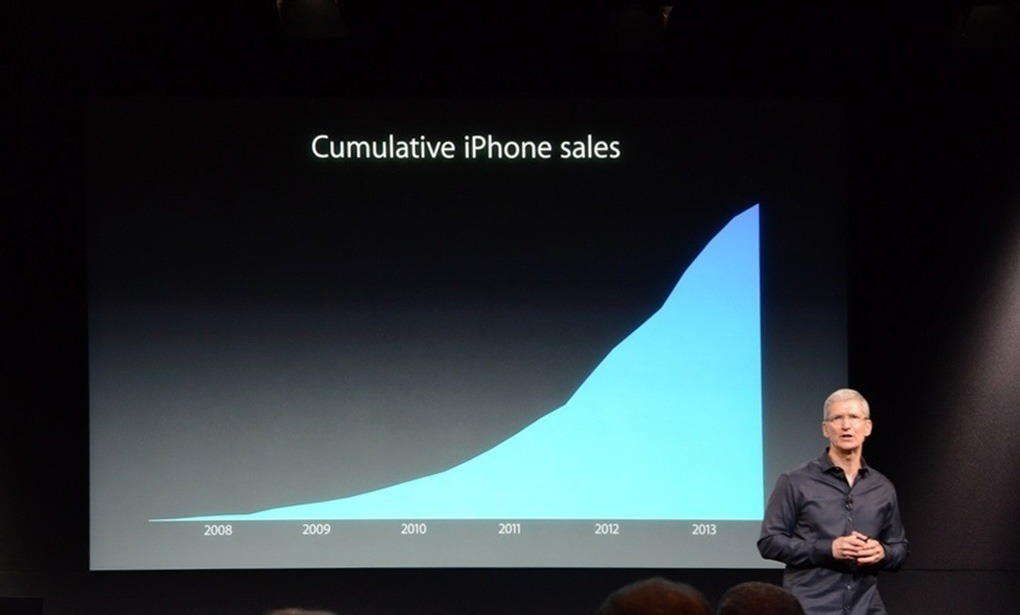
\includegraphics[width=4.5in, trim=1in 0.5in 1.25in 1.25in, clip]{images/iphone-sales.jpg}
    % https://www.techjunkie.com/tim-cook-trying-prove-meaningless-chart/
  \end{center}
  One problem with the graph is that the vertical axis isn't labeled!
  The vertical axis represents the number of iPhones sold since the
  iPhone was first released in 2007. The highest value shown is about
  400 million iPhones.

  Let $f(t)$ be the number of iPhones sold between 2007 and time $t$,
  where $t$ is measured in years.

  \begin{enumerate}
  \item

    \begin{grading}
      1 point
    \end{grading}

    \begin{problem}[\vfill\newpage]
      What does $f'(2010)$ represent? Include units in your answer. 
    \end{problem}

    \begin{solution}
      $f'(2010)$ represents the 
      instantaneous rate of change of the number of iPhones sold with respect to time in 2010. The units
      would be iPhones per year.
    \end{solution}

  \item

    \begin{grading}
      2 points. The important thing is that the graph of $f'$ should be positive and  non-increasing.

      Students might notice that the graph of $f$ looks like it has some sharp corners and draw $f'$ as discontinuous, or they might smooth out the graph; either is fine. 
    \end{grading}

    \begin{problem}[\vfill]
      Let's focus on the last year or so of iPhone sales, just the times to the right of the dashed line below:
      \begin{center}
        \begin{tikzpicture}
          \draw (0, 0) node[anchor=south west]
          {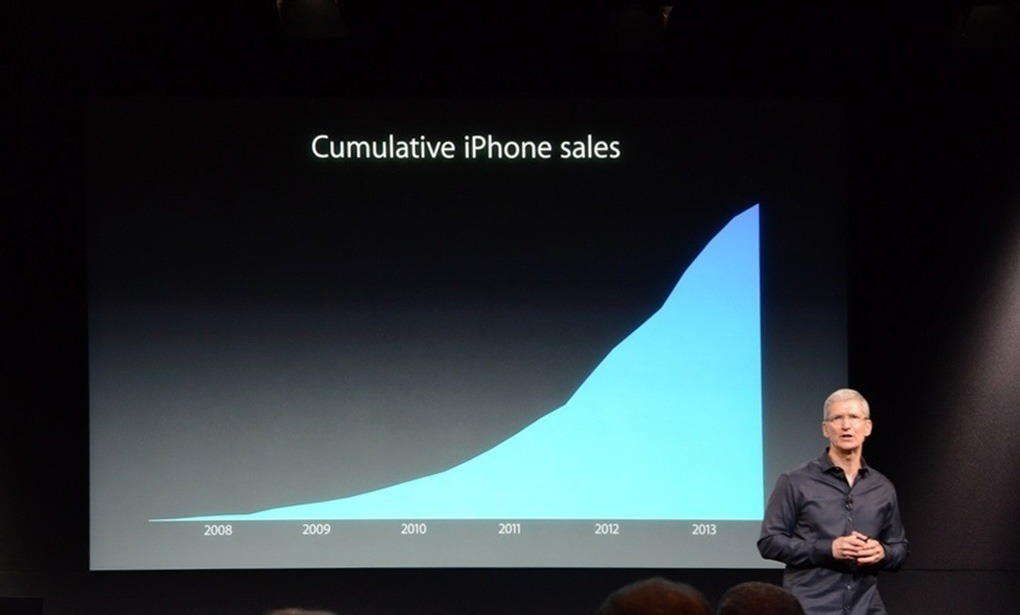
\includegraphics[width=5in, trim=1.75in 1in 3.25in 2.5in, clip]{images/iphone-sales.jpg}
};
          \draw[red, thick, dashed] (10.55, 0.6) -- +(-0.0795, 4.2); 
        \end{tikzpicture}
      \end{center}
      For this time interval, sketch a rough graph of $f'(t)$. We don't have enough information to get a super accurate graph, but aim for the right qualitative behavior and make sure to label your axes.
    \end{problem}

    \begin{solution}
      If you look very closely, it looks like the graph of $f$ is piecewise linear, with perhaps 3 pieces on the interval we're interested in. Each piece is increasing but less steep than the piece before, so one possible graph of $f'$ is something like this:
      \begin{center}
        \begin{tikzpicture}
          \begin{axis}[ymin=0, ytick=\empty, xtick=\empty, hide y axis, width=2.5in]
            \addplot+[sharp plot] coordinates {(0, 47.789) (1, (47.789)}; %
            \addplot+[sharp plot] coordinates {(1, 30) (3, 30)}; %
            \addplot+[sharp plot] coordinates {(3, 16) (3.5, 16)}; %
            \addplot+[open] coordinates {(0, 47.789) (1, 47.789) (1, 30) (3, 30) (3, 16) (3.5, 16)}; %
          \end{axis}
        \end{tikzpicture}
      \end{center}
      It's also reasonable to pretend that the graph doesn't have corners. In that case, we can see that $f$ is increasing and concave down, so $f'$ should be positive and decreasing. So, a graph like this would be plausible:
      \begin{center}
        \begin{tikzpicture}
          \begin{axis}[ymin=0, xtick=\empty, ytick=\empty, hide y axis, width=2.5in]
            \addplot+[domain=0:90]
            {2.6803604618441983/x^0.2378120094247559}; 
          \end{axis}
        \end{tikzpicture}
      \end{center}
    \end{solution}

  \item

    \begin{grading}
      2 points. Any thoughtful answer gets full credit. 
    \end{grading}

    \begin{problem}[\nstretch{0.75}]
      Why do you think Tim Cook might not have wanted to show the graph of $f'$ and instead chose to show the graph of $f$? 
    \end{problem}

    \begin{solution}
      I don't know for sure, but here's my guess. The graph of $f'$ makes it more obvious that the rate of iPhone sales has been decreasing recently. That's not as obvious in the graph Cook decided to show. 
    \end{solution}

  \end{enumerate}

\item \label{gottlieb-5.4.10}

  % based on Gottlieb 5.4.10

  \emph{Interpreting derivatives is very important when applying calculus to other fields; this problem is additional practice with that.}

  Suppose that $C(s)$ gives the number of calories per hour that an average adult burns by walking at a steady speed of $s$ miles per hour (mph).
  \begin{enumerate}
  \item
    \begin{grading}
      1 point. They should also get full credit if they say calories per mile. 
    \end{grading}

    \begin{problem}[0.2in]
      What are the units of $C'(2)$?
    \end{problem}

    \begin{solution} % Jason Bland
      Since the units of $C$ are calories per hour and the units of $s$ are mph, the units of $C'(2)$ are \fbox{calories per hour per mph}. It is possible to ``simplify'' the units: $\displaystyle \frac{\text{calories} / \text{hour}}{\text{miles} / \text{hour}} = \frac{\text{calories}}{\text{mile}}$, but it's actually easier to interpret the derivative if we think of the units as calories per hour per mph.
    \end{solution}

  \item

    \begin{grading}
      1 point
    \end{grading}

    \begin{problem}[\vfill]
      Do you expect $C'(2)$ to be positive or negative? Why?
    \end{problem}

    \begin{solution} 
      We expect $C(s)$ to be an increasing function: moving at a faster speed should burn more calories per hour. Therefore, $C'(2)$ should be \fbox{positive} (any tangent line to an increasing graph has positive slope).
    \end{solution}

  \item \label{gottlieb-5.4.10-estimate}

    \begin{grading}
      2 points
    \end{grading}

    \begin{problem}[\vfill]
      Suppose that an average adult walking at 3 mph burns 320 calories per hour. If $C'(3) = 90$, give an estimate for the number of calories per hour that an average adult walking at 2.9 mph burns. Explain how you obtain your estimate.
    \end{problem}

    \begin{solution}
      The fact that $C'(3) = 90$ says that, when the speed is 3 mph, the instantaneous rate of increase in calories burned per hour is 90 calories per hour per mph. So, if the speed is decreased from 3 mph to 2.9 mph (a change of $-0.1$ mph), we expect the change in calories burned to be about (90 calories per hour / mph)($-0.1$ mph) = $-9$ calories per hour. That is, we expect an average adult walking at 2.9 mph to burn about 9 calories per hour \emph{fewer} than an average adult walking at 3 mph. Therefore, an adult walking at 2.9 mph should burn about $320 - 9 = \boxed{311}$ calories per hour.
    \end{solution}

  \item \label{gottlieb-5.4.10-concavity}

    \begin{grading}
      1 point
    \end{grading}

    \begin{problem}[\vfill\newpage]
      If you also know that the graph of $C(s)$ is concave down, was your estimate in \ref{gottlieb-5.4.10-estimate} an overestimate or underestimate? Explain.
    \end{problem}

    \begin{solution} % Jason Bland
      The estimate gives the value of the line tangent to $C(s)$ at $(3, 320)$ at $s = 2.9$. Since the graph of $C(s)$ is concave down, the tangent line lies above the graph of $C$, so the estimate is an \fbox{overestimate}.
    \end{solution}

  \end{enumerate}

\item  Exam 1 is on Thursday 10/10. Please read {the information on Canvas about the exam}, as well as this \href{https://people.math.harvard.edu/~jjchen/mathma/sample-study-plan.html}{sample study plan}.

  Because this exam covers significantly more material than the mini-exam, it's important to plan out your studying in advance. When making plans, it's easy for people to overestimate their productivity and to be overly optimistic about how much they can accomplish in a given amount of time. In this exercise, we'll have you create a study plan using a process called backward planning; research shows that \href{https://www.cambridge.org/core/journals/judgment-and-decision-making/article/backward-planning-effects-of-planning-direction-on-predictions-of-task-completion-time/92802E42B5A5D987CAADA7F582C2AE0F}{backward planning helps people create more realistic and effective plans}.

  \begin{enumerate}
  \item

    \begin{grading}
      1.5 points, full credit for any reasonable effort
    \end{grading}

    \begin{problem}[\vfill\newpage]
      First, make a to-do list of everything you’d like to do to prepare for the exam, and write your list below. This is likely going to be too long, so identify which items are MUSTs and which are things you'll do only if you have time.

      This list should be focused on active and iterative studying activities. This means it should consist of active styles of review (self-testing and problem solving) over passive styles of review (reading, highlighting, watching lecture videos at 2x speed). As you begin studying, you should update your list based on how your studying goes. 
    \end{problem}

  \item

    \begin{grading}
      1.5 points, full credit for any reasonable effort
    \end{grading}

    \begin{problem}[\vfill\newpage]
      Now, look ahead at your calendar, and lay the tasks from your to-do list into your schedule in reverse order, working backwards from our exam date (Thursday 10/12). For example, if I want to take the first practice exam, then review and visit office hours/MQC, then take the next practice exam, then review and visit office hours/MQC, I might come up with this schedule:
      \begin{itemize}[nosep]
      \item Thursday 10/10: Test day!
      \item Wednesday 10/9: Go to office hours with final questions
      \item Tuesday 10/8: Nothing
      \item Monday 10/7: Take practice exam 2 (timed) and review
      \item Sunday 10/6: Go to MQC with questions from practice exam 1
      \item Saturday 10/5: Check practice exam 1 work against solutions, review topics that were difficult
      \item Friday 10/4: Nothing
      \item Wednesday 10/2 and Thursday 10/3: Take Practice Exam 1
      \end{itemize}
      A few tips:
      \begin{itemize}[nosep]
      \item Try not to put tasks on the test date (and if you have enough time, leave the day before empty too!). You can dip into the test date as an emergency, but not as your plan.
      \item Don't put as many tasks on really busy days (when you have a lot of work or obligations). Again, these are doable as an emergency, but not as your actual plan.
      \item If you can't fit all of your tasks into your schedule, your list of tasks is too ambitious; go back and streamline it right now! Decide what to prioritize, focusing on the most important topics and the study strategies that will most improve your understanding.
      \end{itemize}
      Write your planned schedule below.
    \end{problem}

  \end{enumerate}

\end{enumerate}
\renewcommand{\psrnewpage}{{\centering\rule{5in}{0.4pt}}}

\psreflection{For next class, read \S 5.3, 10.2.}
\end{document}
